\documentclass[11pt]{article}

\usepackage[margin=1in]{geometry}
\usepackage{amsmath}
\usepackage{graphicx}
\usepackage{booktabs}
\usepackage{hyperref}
\usepackage{caption}
\usepackage{array}
\usepackage{siunitx}

\hypersetup{
    colorlinks=true,
    linkcolor=black,
    citecolor=black,
    urlcolor=blue,
    pdftitle={Substitution and Complementarity Between Machine Translation and Generative AI: An Attention-Based Analysis},
    pdfauthor={}
}

\title{Substitution or Complementarity? An Attention-Based Empirical Analysis of Google Translate and ChatGPT Usage Patterns}
\author{Rahman Aliyev\\ University of Pisa\\ Data Science and Business Informatics}

\date{July 2026}

\begin{document}

\maketitle

\begin{abstract}
This report examines whether the emergence of general-purpose generative AI systems, 
exemplified by ChatGPT, has substituted for or complemented dedicated machine translation (MT) tools, exemplified by Google Translate. Using a multi-source attention dataset assembled from Google Trends search indices, Wikipedia pageview counts, and Google Play Store review volumes for Google Translate, ChatGPT, and DeepL, we construct a monthly master panel spanning the period surrounding ChatGPT's November 2022 release. A segmented linear regression of the Google Translate search index around the ChatGPT release date shows a shallower rate of decline in the post-release period (slope = $-0.0751$, intercept = $11.79$) relative to the pre-release period (slope = $-0.1050$, intercept = $21.84$), indicating a downward level shift concentrated at the release date rather than an acceleration of decline. Time-lagged cross-correlation between the two search series is consistently negative across a $\pm 6$-month window (approximately r $-0.61$ to $-0.65$), with the strongest negative association at the 
most negative lags examined. A relative attention-share decomposition places ChatGPT at roughly 
87 percent of combined search interest among the three entities by mid-2026, against approximately 11 percent for Google Translate and 2 percent for DeepL. We argue that these results are best interpreted as evidence of a reallocation of \emph{search attention}, not of absolute user abandonment, and we detail why Google Trends-based indices cannot be read as market share. The report closes with a discussion of the dataset's limitations and 
directions for future work using first-party telemetry. \end{abstract}

\section{Introduction and Research Question}

Google Translate has operated as the dominant free machine translation service since its public launch in 2006, and its 2016 transition to a neural machine translation (NMT) architecture materially improved output fluency and adoption, contributing to a user base reported to exceed one billion monthly active users. For over a decade, the product's growth trajectory was consistent with the demand for translation as a standalone task: users navigated to a dedicated site or application, or used a browser-integrated widget, to convert text or speech from one language to another.

The public release of ChatGPT in November 2022 introduced a different interaction model. Rather than a task-specific tool, ChatGPT is a general-purpose conversational system that can perform translation as one of many capabilities, alongside summarization, drafting, and question answering. Because translation is not ChatGPT's primary marketed function, its effect on dedicated MT tools is not obvious a priori: a user might substitute a general-purpose chat interface for translation tasks entirely, or might treat the two as complements, using ChatGPT for nuanced or context-dependent language work while retaining Google Translate for quick, high-volume, or embedded translation needs.

This report investigates the following research question: \textit{Does the emergence and growth of generative AI, as proxied by public attention to ChatGPT, substitute for or complement public attention to dedicated machine translation tools such as Google Translate?} We approach this question empirically using three independent, publicly observable attention proxies rather than internal usage telemetry, which is not available to us. We treat the analysis as a study of \emph{search and discovery attention}, and we are explicit throughout about the boundaries of what such proxies can and cannot establish about underlying product usage.

\section{Data and Methodology}

\subsection{Data Sources}

Three independent data streams were collected to proxy public attention and engagement with Google Translate, ChatGPT, and DeepL:

\begin{enumerate}
    \item \textbf{Google Trends search indices.} Relative search interest over time for the terms "Google Translate," "ChatGPT," and "DeepL" was collected both programmatically, via an automated extraction script, and through manually exported CSV files covering longer historical windows (a five-year export and a 2016-onward export) where automated access was rate-limited or unavailable. The manual exports were parsed separately and merged with the programmatic extraction on the shared date field.
    \item \textbf{Wikipedia pageview counts.} Monthly pageview counts were retrieved via the Wikipedia pageviews API for the articles \textit{Google\_Translate}, \textit{DeepL}, \textit{ChatGPT}, and \textit{Neural\_machine\_translation}, yielding 133, 102, 44, and 131 monthly records respectively. Wikipedia pageviews serve as a proxy for informational curiosity and brand awareness that is largely independent of Google's search-ranking and query-normalization behavior, providing a partial cross-check on the Trends-based series.
    \item \textbf{Google Play Store review volume.} Review text and metadata were scraped for the corresponding Android applications (\texttt{com.google.android.apps.translate}, \texttt{com.deepl.mobiletranslator}, \texttt{com.openai.chatgpt}), with 2,000 reviews retrieved per application (6,000 rows total). Review volume and timing serve as a coarse proxy for active engagement, distinct from search-based discovery.
\end{enumerate}

\subsection{Extraction Pipeline}

Data collection was implemented as a sequence of discrete, auditable scripts rather than a single monolithic process, so that each source could be re-run or debugged independently:

\begin{itemize}
    \item \texttt{01\_extract\_google\_trends.py} performed the automated Google Trends extraction and produced an initial cleaned dataset and diagnostic plot.
    \item \texttt{01b\_parse\_manual\_trends\_export.py} parsed the manually exported Trends CSV files (\texttt{multiTimeline\_2016.csv.csv}, 127 rows, and \texttt{multiTimeline\_5\_years.csv}, 262 rows) and merged them on the date column, producing a combined file of 380 rows. Because the two exports had partially overlapping date ranges and column sets, the merge produced suffixed duplicate columns (e.g., \texttt{ChatGPT\_x}, \texttt{ChatGPT\_y}) that required subsequent reconciliation.
    \item \texttt{02\_extract\_wikipedia\_pageviews.py} retrieved the Wikipedia pageview series described above, producing 410 combined rows.
    \item \texttt{03\_extract\_app\_reviews.py} retrieved the Play Store review data described above, producing 6,000 combined rows.
    \item \texttt{04\_merge\_and\_process.py} merged the cleaned Trends, Wikipedia, and review-derived series into a single master dataset of 664 rows.
    \item \texttt{05\_analyze.py} performed the segmented regression, cross-correlation, and relative-attention-share analyses reported in Section~\ref{sec:findings}.
\end{itemize}

\subsection{Pre-processing}

Several pre-processing steps were necessary before the merged data could support analysis:

\begin{itemize}
    \item \textbf{Numeric normalization of Trends values.} Google Trends reports values below 1 as the string \texttt{"<1"} rather than a numeric value. These entries were converted to \num{0.5} as a conservative midpoint, and all remaining values were coerced to numeric type, with non-parseable entries set to zero.
    \item \textbf{Column unification across languages.} Because part of the manual export data originated from a non-English-language locale, the Google Translate series appeared under a localized Russian-language label ("Google Translator," transliterated) in addition to its English label. A rename map consolidated all locale-specific and merge-suffixed variants (\texttt{\_x}/\texttt{\_y}) of each entity name into a single canonical column per entity.
    \item \textbf{Duplicate column reconciliation.} Following the rename step, columns sharing a canonical name were grouped and reduced to a single series per entity, first by taking the first non-null value and, where duplicates persisted after this step, by averaging across the duplicate columns.
    \item \textbf{Resampling to monthly frequency.} All three source series (Trends, Wikipedia pageviews, and review counts) were aligned to a common monthly time index to permit direct comparison and merging into the master dataset.
\end{itemize}

The resulting master dataset (\texttt{./data/master\_dataset.csv}, 664 rows) forms the basis for the empirical analysis in Section~\ref{sec:findings}.

\section{Empirical Analysis and Findings}
\label{sec:findings}

\subsection{Segmented Linear Regression: Pre- vs. Post-ChatGPT Trend}

To evaluate whether the release of ChatGPT coincided with a change in the trajectory of search attention toward Google Translate, we fit separate ordinary least squares regressions of the Google Translate Trends index on a monthly time index, split at the ChatGPT release date (November 2022). Table~\ref{tab:segmented} reports the estimated slope and intercept for each segment.

\begin{table}[htbp]
\centering
\caption{Segmented regression of the Google Translate search index}
\label{tab:segmented}
\begin{tabular}{lccc}
\toprule
Segment & Slope & Intercept & $n$ (months) \\
\midrule
Pre-ChatGPT  & $-0.1050$ & $21.84$ & 82 \\
Post-ChatGPT & $-0.0751$ & $11.79$ & 45 \\
\bottomrule
\end{tabular}
\end{table}

Two features of this result are worth separating. First, the intercept drops sharply between segments, from approximately 21.8 to 11.8, indicating a level shift: the average search index for Google Translate is markedly lower in the months immediately surrounding and following the ChatGPT release than the pre-period trend would have predicted. Second, the slope in the post-ChatGPT segment ($-0.0751$) is smaller in magnitude than the pre-ChatGPT slope ($-0.1050$), meaning that the \emph{rate} of decline in Google Translate search interest is not accelerating after ChatGPT's release; if anything, the post-period decline is somewhat gentler. Taken together, these two facts are consistent with a one-time downward repositioning of Google Translate's search attention baseline around the emergence of ChatGPT, rather than a continuously steepening erosion driven by ongoing generative AI adoption. This distinction matters for interpretation: a steepening slope would suggest an accelerating substitution process, whereas a level shift with a stable or flattening slope is more consistent with a discrete reallocation of attention that has since stabilized at a new, lower baseline.

\subsection{Time-Lagged Cross-Correlation}

To characterize the temporal relationship between attention to ChatGPT and attention to Google Translate, we computed the Pearson cross-correlation between the two monthly Trends series across lags from $-6$ to $+6$ months, where a positive lag indicates ChatGPT search interest leading Google Translate search interest by that many months. Results are reported in Table~\ref{tab:crosscorr}.

\begin{table}[htbp]
\centering
\caption{Time-lagged cross-correlation between Google Translate and ChatGPT search indices}
\label{tab:crosscorr}
\begin{tabular}{cc}
\toprule
Lag (months) & Correlation ($r$) \\
\midrule
$-6$ & $-0.6475$ \\
$-5$ & $-0.6404$ \\
$-4$ & $-0.6347$ \\
$-3$ & $-0.6299$ \\
$-2$ & $-0.6248$ \\
$-1$ & $-0.6188$ \\
$0$  & $-0.6128$ \\
$1$  & $-0.6030$ \\
$2$  & $-0.5914$ \\
$3$  & $-0.5786$ \\
$4$  & $-0.5668$ \\
$5$  & $-0.5552$ \\
$6$  & $-0.5482$ \\
\bottomrule
\end{tabular}
\end{table}

The correlation is negative across the entire lag window examined, ranging from approximately $-0.55$ to $-0.65$. Two aspects of the lag structure are notable. First, the magnitude of the negative correlation is not constant: it is strongest (most negative, $r=-0.6475$) at $\text{lag}=-6$, where Google Translate search interest six months earlier is being compared with current ChatGPT interest, and weakens monotonically as the lag moves toward $+6$. Second, the correlation is negative even at lag zero ($r=-0.6128$), indicating substantial \emph{contemporaneous} inverse co-movement rather than a relationship that only emerges with a delay.

The pattern of a strong, front-loaded negative association that decays gradually toward more positive lags is consistent with a relatively short substitution lag: shifts away from Google Translate search interest are associated with contemporaneous or near-contemporaneous increases in ChatGPT search interest, rather than with a delayed response measured in many months. However, we note that Google Trends indices are relative and internally re-normalized measures, and both series exhibit strong underlying time trends (Google Translate declining, ChatGPT rising) over the sample window; a substantial share of the observed cross-correlation may therefore reflect these opposing trends rather than a tight causal lead-lag relationship at any single lag. We treat the cross-correlation results as descriptive evidence of association, not as an identified causal estimate of substitution timing.

\subsection{Relative Attention Share}

Finally, we computed each entity's share of combined search interest among the three entities, by month, over the most recent months in the sample. Table~\ref{tab:relshare} reports these shares, and Figure~\ref{fig:relshare} presents them graphically as a stacked area chart.

\begin{table}[htbp]
\centering
\caption{Relative share of search attention across entities, most recent months}
\label{tab:relshare}
\begin{tabular}{lccc}
\toprule
Month & ChatGPT & DeepL & Google Translate \\
\midrule
2026-03 & 0.8571 & 0.0179 & 0.1250 \\
2026-04 & 0.8611 & 0.0185 & 0.1204 \\
2026-05 & 0.8624 & 0.0183 & 0.1193 \\
2026-06 & 0.8679 & 0.0189 & 0.1132 \\
2026-07 & 0.8700 & 0.0200 & 0.1100 \\
\bottomrule
\end{tabular}
\end{table}

\begin{figure}[htbp]
\centering
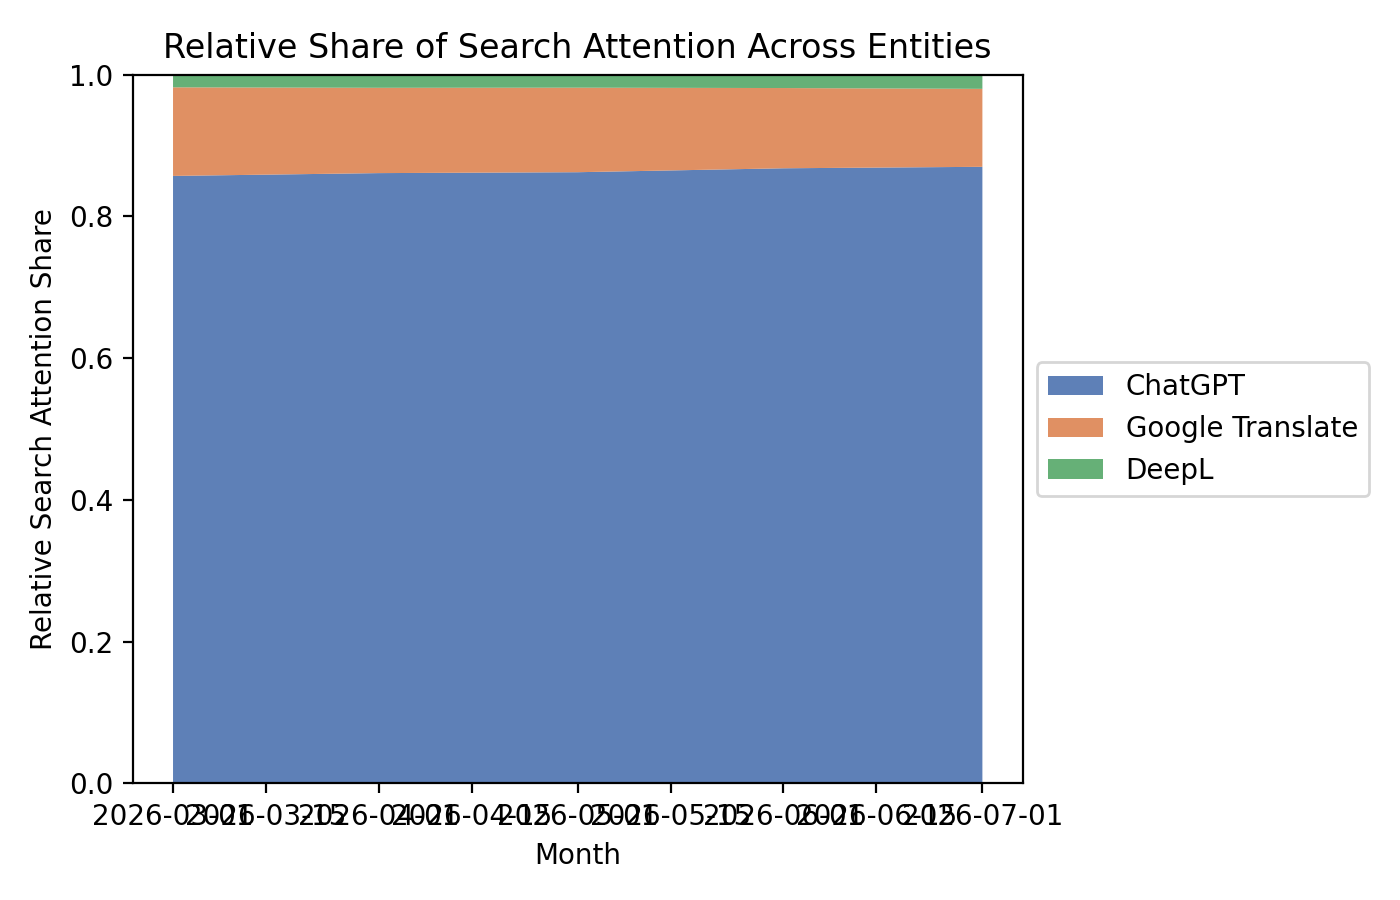
\includegraphics[width=0.75\textwidth]{./relative_share.png}
\caption{Relative share of search attention across ChatGPT, Google Translate, and DeepL, by month.}
\label{fig:relshare}
\end{figure}

By the most recent month in the sample (July 2026), ChatGPT accounts for approximately 87 percent of combined search interest across the three entities, against approximately 11 percent for Google Translate and 2 percent for DeepL. The share attributable to ChatGPT rises modestly but consistently across the five months shown, while Google Translate's share declines by a corresponding amount; DeepL's share is comparatively stable and small throughout.

\section{Methodological Caveat: Search Attention Share Is Not Market Share}
\label{sec:caveat}

The relative-attention-share figures in Section~\ref{sec:findings} require careful interpretation, and we treat this distinction as central to the report rather than a minor caveat.

Google Trends indices measure the relative volume of a specific search query against the maximum search volume for that query within the selected time window and region; they are re-normalized to a 0--100 scale and are not comparable to absolute query volume, let alone to product usage. A search attention share of 87 percent for ChatGPT does not imply that ChatGPT is used for 87 percent of translation-related tasks, or that Google Translate retains only a comparably small fraction of its user base. It indicates only that, among explicit navigational or informational searches for these three brand names, ChatGPT-related queries currently make up the large majority.

This distinction is material because Google Translate's usage pattern differs structurally from a typical search-driven product. Google Translate is reported to serve over one billion monthly active users, a substantial share of whom reach the service through channels that do not register as a branded search query at all: the integrated translation widget in the Chrome browser, the "Translate this page" prompt on non-native-language web pages, in-page translation in Gmail and Google Search results, and direct app or extension usage that a returning user reaches without searching for the brand name each time. A user who translates a web page daily via a browser-integrated widget contributes zero observations to the Google Trends series for "Google Translate," while a user who is curious about ChatGPT and searches for it by name multiple times in a research or evaluation period contributes multiple observations to the ChatGPT series. The two products are not equally exposed to search-based measurement, and this asymmetry biases any naive comparison of Trends-derived shares toward understating Google Translate's absolute usage and overstating ChatGPT's usage relative to it.

Wikipedia pageviews and Play Store review counts, the two supplementary series collected in this study, partially mitigate this concern insofar as they capture informational curiosity and active app engagement rather than pure search behavior, but both remain proxies for attention and discovery rather than direct usage telemetry, and neither was incorporated into the headline regression or cross-correlation results reported above. We therefore characterize the findings of this report as evidence about the reallocation of public \emph{search and discovery attention} toward generative AI and away from dedicated translation tools, and explicitly do not characterize them as evidence about the reallocation of absolute product usage or market share.

\section{Conclusion and Limitations}

The empirical results in this report are consistent with a measurable, structural shift in public search attention toward generative AI and away from dedicated machine translation search around the release of ChatGPT: a lower post-release intercept in the segmented regression, a persistently negative cross-correlation between the two series across the lag window examined, and an attention-share decomposition in which ChatGPT now accounts for the large majority of combined search interest among the three entities studied. Taken together, these patterns support the substitution hypothesis at the level of search behavior: when users search for translation-adjacent tools by name, they are increasingly searching for ChatGPT rather than Google Translate or DeepL.

At the same time, as discussed in Section~\ref{sec:caveat}, this evidence is bounded by what search-based proxies can establish. It does not, on its own, demonstrate that generative AI has displaced dedicated translation tools in absolute usage, given Google Translate's large embedded and widget-based user base that does not generate branded search queries. The dataset is further limited in several respects that should inform future work:

\begin{itemize}
    \item \textbf{Reliance on third-party proxies.} All three data sources (Google Trends, Wikipedia pageviews, Play Store reviews) are external proxies for attention and engagement rather than first-party product telemetry such as daily or monthly active users, session counts, or task-level usage logs, none of which are publicly available for either product.
    \item \textbf{Locale and query-normalization sensitivity.} The need to reconcile a Russian-language localized query label for "Google Translate" during pre-processing illustrates a broader limitation: Google Trends results are sensitive to region, language locale, and query normalization choices in ways that can affect merged multi-region series if not carefully handled.
    \item \textbf{Correlational, not causal, design.} The cross-correlation analysis is descriptive; both series exhibit strong opposing trends over the sample period, and the analysis does not isolate a causal substitution effect net of these trends.
    \item \textbf{Review volume as an engagement proxy.} Play Store review counts were collected but not incorporated into the headline regression and correlation analyses; a more complete treatment would model review volume and sentiment jointly with the search-based series.
\end{itemize}

Future work should, where possible, incorporate first-party or panel-based usage data (e.g., comScore- or Similarweb-style panel measurement, or app-analytics platforms with cross-app session data) to distinguish search-attention substitution from usage-level substitution, extend the analysis to non-English-language markets where Google Translate's embedded-usage advantage may be more or less pronounced, and apply formal structural-break tests (e.g., a Chow test or Bai-Perron procedure) to the segmented regression to assess the statistical significance of the observed level shift rather than reporting point estimates alone.

\end{document}
